\documentclass[10pt,journal,compsoc]{IEEEtran}
\usepackage{blindtext}
\usepackage{multicol}
\usepackage{listings}
\usepackage{graphicx}
\usepackage{wrapfig}
\usepackage{float}
\graphicspath{ {./images/} }
\usepackage[english]{babel}

\usepackage{graphicx} % package for including graphics
\usepackage{amsmath} % package for using mathematical symbols
\usepackage{amssymb} % package for using additional mathematical symbols
\usepackage{subfig} % package for including multiple figures on one page
\usepackage{url}
\usepackage{booktabs}
\usepackage{tabularx}
\usepackage[hidelinks]{hyperref}
\usepackage{color}

\usepackage{xcolor}
\usepackage{float}
\usepackage{graphicx}
\usepackage[utf8]{inputenc}
\usepackage{shortcut}
\usepackage{enumitem}

\usepackage{array}
\usepackage{multirow}
\usepackage{multicol}
\usepackage{boldline}
\usepackage{hhline}

\begin{document}

\definecolor{azulUC3M}{RGB}{0,0,102}

\begin{titlepage}
    \begin{sffamily}
        \color{azulUC3M}
        \begin{center}
            \begin{figure}[H] %incluimos el logotipo de la Universidad
                \makebox[\textwidth][c]{
\includegraphics[width=16cm]{Portada_Logo.png}}
            \end{figure}
            \vspace{2.5cm}
            \begin{Large}
                Master in Cybersecurity\\
                2022-2023\\
                \vspace{2cm}
                \textsl{Master's Thesis}
                \bigskip

            \end{Large}
            {\Huge \textbf{``Secure speedup of the future JavaScript deployments''}\\
            \vspace*{0.5cm}
            \rule{10.5cm}{0.1mm}\\
            \vspace*{0.9cm}
            }
            {\LARGE {Aitor Ruiz Garcia}\\
            \vspace*{1cm}
            }
            \begin{Large}
                Director\\
                Pedro Peris López\\
                Madrid, 2023\\
            \end{Large}
        \end{center}
        \vfill
        \color{black}
        
\includegraphics[width=4.2cm]{creativecommons.png}\\
        Esta obra se encuentra sujeta a la licencia Creative Commons \textbf{Reconocimiento - No Comercial - Sin Obra Derivada}\\
    \end{sffamily}
\end{titlepage}

\title{Secure speedup of the future JavaScript deployments}
\author{\IEEEauthorblockN{Aitor Ruiz Garcia*}\\
    \IEEEauthorblockA{\textit{Master in Cybersecurity, Universidad Carlos III de Madrid}}
    \thanks{*Corresponding author.}% <-this % stops a space
    \thanks{\textit{E-mail address:}100482217@alumnos.uc3m.es}}

\date{September 2023}
\maketitle
\section{Abstract}
JavaScript has emerged as a fundamental language in global development. Much of the success of Node.js, both in server-side applications and in full-stack web applications (client-server), can be attributed to this language.

Node.js was primarily created to enable JavaScript to run on the server. The creator of Node never anticipated that JavaScript would be used for virtually everything.

JavaScript is employed in desktop applications using Electron \cite{ELECTRON}, and in mobile applications using React Native \cite{RN} or Ionic \cite{IONIC}. Being an interpreted language, it offers a low entry barrier. As the default language of the web, it also boasts a plethora of compelling libraries.

Node.js took the V8 engine, which runs JavaScript on Chrome, and wrapped it in additional C++ code to enable it to interact with system calls \cite{FKNODE}.

All these factors have contributed to the ascent of JavaScript as the language of the future. Nonetheless, as the creator himself has stated, the language has experienced some 'growing pains' \cite{FKNODE}.

This project is conceived with the aim of addressing some of these challenges. The primary objective is to develop a library for Deno projects to accelerate the most frequent operations. This library will be crafted in Rust, a language renowned for its speed and memory safety.

The targeted operations are cryptographic ones, such as hashing, encrypting, and decrypting. These operations are prevalent in the web domain and demand significant CPU resources. This makes them ideal candidates for this project.

\section{The problem}

Ryan Dahl, the creator of Node.js, has expressed his regrets about the language \cite{FKNODE}. He has stated that he would not use JavaScript for a new project and that he would also not use Node.js for a new project. Node.js has grown beyond its original intentions and has become a 'monster'.

While experimenting with the TFG \cite{TFG} project, some problems were encountered with the current state of the JavaScript ecosystem. These issues will be explained in the following sections. The TFG project was a web application with blockchain integrations for decentralized identity management. Although this project is not within the scope of this TFM, understanding its context is crucial to grasp the problems that were discovered.


\subsection{No types}
JavaScript does not have a type checker, at least not at \textit{compile} time. Since JavaScript is an interpreted language, it lacks a compile step. This absence means there isn't a compiler to validate the types of variables, allowing a value of one type to be assigned to a variable of another type. Such assignments can lead to unforeseen errors in the code. Additionally, one might attempt to access a property of an object that does not exist, resulting in a runtime error without prior warning.

Consider the following example:
\begin{lstlisting}
const user = {
    name: "",
    age: 0
}
    
console.log(user.email);
\end{lstlisting}

This snippet will not alert the developer to the fact that the user object lacks an email property, leading directly to a runtime error, which detracts from the developer experience.

It becomes even more problematic when end-users encounter this error in a production environment. They would be presented with an error they can't comprehend.

Such issues arise because JavaScript is a dynamic language that lacks a built-in type checker.

The original TFG \cite{TFG} utilized Next.js, a renowned framework for server-rendered React applications. At the project's inception, the complications detailed in the following sections weren't anticipated. Next.js was the framework of choice due to its familiarity. As the project progressed, however, challenges emerged, most notably concerning the lack of type-checking.

\subsection{node\_modules}

Node.js features a package manager named npm. This manager facilitates the installation of libraries into a project. However, a predicament arises due to these libraries being saved in the \verb|node_modules| directory, which can bloat considerably over time. \cite{BADNPM}

By default, npm does not create symbolic links between libraries. Consequently, if two libraries rely on the same dependency, that dependency will be duplicated within the installation. Having more packages means greater disk space consumption and extended installation times. As a result, a CI build could spend a significant duration merely installing all the requisite packages.


\subsubsection{node\_modules security implications}

As JavaScript is predominantly utilized in web applications, both on the server and client sides, it presents an enticing target for attacks. As of now, npm hosts over 1.6 million packages. \cite{NPMCOUNT}

If an attacker successfully exploits a web framework, they could potentially access a vast number of browsers. Even if only a small fraction of these browsers is vulnerable, the impact can be significant.

While JavaScript in browsers is sandboxed, enhancing its security, the same cannot be said for Node.js. Within Node.js, code has the capability to interact with both the file system and the entire internet.

Historically, there have been several instances of compromised npm packages. Among the most notable are \verb|colors| and \verb|faker.js|. \cite{BADFAKER} \cite{VERGEFAKER}

In these cases, the developer maliciously introduced infinite loops, disrupting the standard workflows of numerous other developers.

Another alarming instance involved \verb|UAParser.js|, which, when downloaded, secretly installed a password stealer and a cryptominer. It's crucial to recognize that this package is still accessed by millions of users on a daily basis.

\subsection{Node GYP}

Node GYP is the state of the art when it comes to creating native libraries in Node.js. This tool originally came from Google \cite{FKNODE}. When Google discontinued it, the community created a fork, allowing the project to continue. \cite{NODEGYP}

It is a tool written in Python, which is not JavaScript, making it unnecessarily complicated to write a native library.

To create a native library, a profound understanding of \verb|C++| is required. The tooling associated with it is written in various languages, adding an extra layer of complexity to the development of native libraries.

In the original repository, a simple example of a native library is presented. \cite{NODEGYP}

This example consists of 33 lines of code for a basic "Hello World".

\begin{lstlisting}
extern "C" NODE_MODULE_EXPORT void
NODE_MODULE_INITIALIZER(
    v8::Local<v8::Object> exports,
    v8::Local<v8::Value> module,
    v8::Local<v8::Context> context) {
  NODE_SET_METHOD(exports, "hello", Method);
}
\end{lstlisting}

A significant amount of boilerplate code is needed just to pinpoint the actual function that will be called from JavaScript.

\begin{lstlisting}
static void Method(
    const v8::
    FunctionCallbackInfo<v8::
    Value>& 
    args
    ) {
  v8::Isolate* isolate = args.GetIsolate();
  args.GetReturnValue()
    .Set(
        v8::String::NewFromUtf8(
        isolate, 
        "world")
        .ToLocalChecked()
    );
}
\end{lstlisting}

Interacting directly with the V8 engine is necessary, which is no simple feat. Although this code appears basic, it is not straightforward. It merely returns a string with the value \verb|world|.

This code would be even more intricate in other C ABI compatible languages because they would need to implement the V8 engine in their native language to communicate with it.

Rust, which will be discussed later, has a crate that directly links with V8. Nevertheless, it remains a challenging task to implement.

\section{The solution}

Ryan Dahl created Deno as a solution to the challenges he faced while working on Node.js without a clear roadmap. In a talk at JSConf \cite{FKNODE}, he introduced the project with a definitive plan to position Deno as the standard language for the web.

His goal was to craft a safe and secure environment for JavaScript and TypeScript execution. This would mean that developers wouldn't need to fret about security issues since the code would run within a sandboxed environment.

By default, Deno is designed to restrict access to both the file system and the internet. Given that JavaScript inherently operates within a sandboxed environment, this move is a logical progression.

Deno's architecture relies on message passing between the host and the sandboxed environment, eliminating the host's direct access to the latter. This is a commendable security feature as it prevents the host from infiltrating the sandboxed environment. Such a setup simplifies embedding Deno into other projects since developers would only need to implement the message-passing protocol.

The entire experience aims to mirror web interactions closely. On the web, imports are facilitated via URLs, and Deno is intended to function similarly.

The following section highlights some of the solutions that were developed.

\subsection{TypeScript}

TypeScript was introduced in 2012 by Microsoft to augment JavaScript with type capabilities. It operates as a superset of JavaScript, implying that all keywords valid in JavaScript are also valid in TypeScript, but the reverse is not true. \cite{TypeScript} \cite{10162220}

Rather than modifying V8, TypeScript designates JavaScript as the compile target of TypeScript. This strategy allows targeting various versions of JavaScript and incorporating polyfills \cite{Polyfill} if the necessary API is absent.

While TypeScript is undeniably beneficial, it introduces additional time to the development workflow. This is attributed to the need to first compile TypeScript to JavaScript and subsequently execute the program. This sequence is typical for most Node.js projects. The \verb|package.json|, in many cases, is structured as:

\begin{lstlisting}
"scripts": {
    "start": "node index.js",
    "build": "tsc"
}
\end{lstlisting}

This mandates that the developer invoke the \verb|build| script before initiating the \verb|start| script. While this might not pose challenges during development, it can be cumbersome in a production setting, especially since the \verb|build| script needs execution prior to application deployment.

Contrastingly, Deno compiles TypeScript in real-time and forwards it to V8, streamlining the entire process. Developers are spared the hassle of configuring an external utility, since the compiler, \verb|tsc|, can be intricate to install and fine-tune.

In terms of coding, this ensures that every variable possesses a designated type, which remains consistent throughout the code.

\begin{lstlisting}
var name: string = "";
\end{lstlisting}

The variable `name` can't be reassigned with a non-string value.

\begin{lstlisting}
name = 0;
\end{lstlisting}

This snippet would trigger an error since \verb|0| isn't a string.

\subsubsection{JSDoc}

While TypeScript offers a robust solution, its setup can be cumbersome. It demands extensive configuration, making it challenging to integrate into certain projects. Although JSDoc's primary objective is to furnish documentation about functions—enabling developers to understand a function's usage—it can also be harnessed to assign types to variables.

Remarkably, it's feasible to derive TypeScript types from JSDoc annotations.

\begin{lstlisting}
/**
 * @type {string}
 */
var name = "";
\end{lstlisting}

With such a simple annotation, a variable is typed. Armed with this information, a \verb|.d.ts| file can be generated, which `tsc` will then utilize to apply type-checking to native JavaScript code.

Noteworthy projects in this domain include Svelte and Turbo.

\subsubsection{Svelte}

Svelte \cite{10101104} is a framework designed for crafting UIs, similar to React. It stands as an excellent alternative to React due to its speed and reduced bundle size.

In an article, the Svelte author delves into the merits of integrating TypeScript with Svelte. In his opinion, utilizing TypeScript for crafting a framework is "\textit{not worth it}."

He contends that while TypeScript possesses undeniable strengths, the hassle involved in its setup outweighs the benefits, at least in his specific case.

The majority of their challenges arise from the intricacies of generics and the type magic necessary for addressing certain edge cases within their framework.

\textit{''My position is, types are fantastic, TypeScript is a bit of a pain … as soon as you use a .ts file, then you have to have the tooling to support that … there's all of these points of friction when you use a non-standard language like TypeScript that I have come to believe makes it not worth it. So instead, we have put all our types in JSDoc annotations, and we get all of the type safety, but none of the drawbacks, because it is just JavaScript, everything is in comments, you can just run the code. This is what we do in the Sveltekit codebase and it has worked out fantastically so for Svelte 4.0, we're going to do the same for Svelte because it's going to enable us to move much more quickly.''} - \textit{Rich Harris} \cite{SvelteTS}

\subsubsection{Turbo}

Turbo is a library designed to simplify backend development tasks by facilitating the direct insertion of HTML into a page without necessitating a full page reload.

Recently, the library's lead developer and the mind behind Ruby on Rails announced their decision to entirely exclude TypeScript from the project. Consequently, this means any project relying on Turbo will need to adjust since the team does not intend to provide any type information moving forward.

He primarily argues that types compromise code readability and the setup effort isn't justifiable.

\textit{''TypeScript just gets in the way of that for me. Not just because it requires an explicit compile step, but because it pollutes the code with type gymnastics that add ever so little joy to my development experience, and quite frequently considerable grief. Things that should be easy become hard, and things that are hard become `any`. No thanks!''} - \textit{David Heinemeier Hansson} \cite{TurboTS}

\subsubsection{ECMAScript proposal}

There is currently an ECMAScript proposal underway that aims to introduce types to native JavaScript. Although it is still in stage 1 and may remain in this stage for a considerable time, the proposal shows great promise.

The primary advantage is the elimination of build steps. Developers will have access to types directly within JavaScript. This enhancement will bring about the following improvements to the language:

\begin{itemize}
    \item Reduced time spent on build steps.
    \item More streamlined code than JSDoc.
    \item Better code optimization opportunities for engine makers.
\end{itemize}

In the interim, how can we enhance the developer experience?

\subsubsection{How Deno can imporove the TypeScript experience}

Using Deno, there are no more build steps. This means that a developer can write TypeScript and run it directly in Deno. This provides an excellent developer experience, as there's no need to worry about a build step.

Opting out of types in your code is also a valid choice, so Deno permits the execution of plain JavaScript as well. This approach offers the best of both worlds.

When the project's scope is not clearly defined and rapid iterations are desired, JavaScript can be employed. As the concept matures, TypeScript can be integrated.

Many of the issues faced by library authors arise from third-party libraries that are cumbersome to work with. However, Deno has the potential to streamline and enhance this experience.

\subsection{URL based imports}

A significant change in Deno is the adoption of URL-based imports; modules are cached and then reused as required.

However, given that scripts are sourced from URLs, they might contain malicious code. How can developers safeguard themselves?

\subsubsection{Security checks}

Deno implements multiple checks to prevent uncontrolled access to the machine. \cite{DenoSec}

\begin{itemize}
    \item \textbf{--allow-env}: Allows reading of \verb|.env| files.
    \item \textbf{--allow-sys}: Permits reading of system-specific information, such as the OS version or memory details.
    \item \textbf{--allow-hrtime}: Enables high-resolution time measurement. High-resolution time can be exploited in timing attacks and fingerprinting.
    \item \textbf{--allow-net}: Grants network access. An optional, comma-separated list of IP addresses or hostnames (optionally with ports) can be provided to establish an allow-list of permitted network addresses.
    \item \textbf{--allow-ffi}: Permits loading of dynamic libraries. This feature is still in an unstable state.
    \item \textbf{--allow-read}: Authorizes file system read access.
    \item \textbf{--allow-run}: Allows execution of subprocesses.
    \item \textbf{--allow-write}: Grants file system write access.
\end{itemize}

All these flags have opposite counterparts. They can be utilized to authorize access to certain folders while denying access to specific files. For example:

\begin{lstlisting}
--allow-read=/etc \
--deny-read=/etc/hosts
\end{lstlisting}

\subsection{Speedup}

The solution that some project owners have adopted to enhance performance is the use of a compiled language as a companion. These languages, \textit{in general}, exhibit better performance than interpreted ones.

In the realm of web development, two projects particularly stand out. The developer ecosystem surrounding web development has expanded exponentially, and now, more than ever, a bundler \cite{Bundler} is essential to amalgamate all this information into a straightforward blend of HTML, CSS, and JS.

\verb|SWC| and \verb|esbuild| both leverage other languages to achieve speedups. Notably, these two projects played a pivotal role in the development of this project.

\subsubsection{SWC}

SWC (Speedy Web Compiler) is a project that aims to accelerate the compilation of JavaScript and TypeScript. This means it takes an existing TypeScript codebase and converts it to JavaScript, ensuring the output is neat and compact.

Since not all browsers support the latest JavaScript features, SWC can also transpile the code to an older version of JavaScript. The range of browsers that SWC supports is notably extensive.

SWC opted to compile a Rust program into a binary. Subsequently, they wrote some JS glue code to facilitate its use in a JS project.

Given that this application primarily operates as a CLI-style application, this approach is advantageous. This is attributed to the minimal JS code required—essentially, the only task is to relay the necessary arguments to the Rust binary. From there, the Rust program takes the helm and packages the JS application.

However, while this method is apt for the given use-case, it may not be as fitting for a library intended to execute when a developer invokes a function. The glue code would have to spawn a shell, which consumes time. In fact, the delay might be so significant that the benefits of using a native library could be nullified.

\subsubsection{esbuild}

esbuild is a bundler \cite{Bundler} that aspires to be the fastest bundler in the world. A bundler amalgamates all dependencies into a single file for distribution to users. This practice is prevalent in the web space, as it can also segment code into chunks for on-demand loading. Such an approach is particularly beneficial for expansive applications because it can diminish the initial load time, as exemplified by the TFG \cite{TFG} project.

\verb|esbuild| opted for a distinct strategy. They employed wasm \cite{WASM} \cite{WASMSPEC} for crafting the library. Given that this project is penned in Go, the entire Go garbage collector must be integrated into the wasm code.

Such integration can lead to enlarged install sizes and a suboptimal developer experience, as mentioned previously.

It's pivotal to highlight that, although wasm is a commendable technology that has ushered in substantial speed improvements to the web, it still lacks an efficient memory management solution. Consequently, while it offers impressive performance in contrast to JavaScript, it might not fare as well when juxtaposed with other technologies.

\section{The code}
The proposed solution is a dynamic library complemented with minimal TypeScript glue code.

Deno provides exceptional dynamic library support through their native API.

\begin{lstlisting}
Deno.dlopen(
    test.lib,
    {},
)
\end{lstlisting}

Deno is compatible with the complete C ABI, which means it can load any dynamic library adhering to the C ABI standards. This flexibility is beneficial, enabling developers to utilize any language in alignment with the C ABI.

\begin{table}[H]
    \begin{tabular}{|l|l|l|}
        \hline
        \textbf{FFI Type}              & \textbf{Deno}     & \textbf{Rust}     \\ \hline
        i8                             & number            & i8                \\ \hline
        u8                             & number            & u8                \\ \hline
        i16                            & number            & i16               \\ \hline
        u16                            & number            & u16               \\ \hline
        i32                            & number            & i32               \\ \hline
        u32                            & number            & u32               \\ \hline
        i64                            & number | bigint   & i64               \\ \hline
        u64                            & number | bigint   & u64               \\ \hline
        usize                          & number | bigint   & usize             \\ \hline
        f32                            & number | bigint   & f32               \\ \hline
        f64                            & number | bigint   & f64               \\ \hline
        void{[}1{]}                    & undefined         & ()                \\ \hline
        pointer                        & \{\} | null       & *mut c\_void      \\ \hline
        buffer{[}2{]}                  & TypedArray | null & *mut u8           \\ \hline
        function{[}3{]}                & \{\} | null       & Option\textless{} \\
                                       &                   & extern "C" fn()   \\
                                       &                   & \textgreater{}    \\ \hline
        \{ struct: {[}...{]} \}{[}4{]} & TypedArray        & MyStruct          \\ \hline
    \end{tabular}
\end{table}

Considering this project solely involves strings and numbers, the only required types are a pointer and u32. Thus, the dynamic library's type declaration is as follows:

\begin{lstlisting}
hash: {
    parameters: ["pointer", "u32"],
    result: "pointer",
    nonblocking: true,
}
\end{lstlisting}

This specification pertains to the hash function in the library. Within the declaration, one can observe a \verb|nonblocking| flag. This flag informs Deno that the function operates asynchronously. Rather than dealing with intricate C ABI callbacks, Deno seamlessly transforms synchronous Rust code into asynchronous JavaScript code.

Given the inherent asynchronous nature of the Deno ecosystem, all the library's functions are asynchronous. This choice simplifies the developer's tasks, especially since Deno features top-level await. Hence, there's no need to encase the code in promises or callbacks.

The table provided by Deno facilitates the conversion of types from JavaScript to Rust. It incorporates some Rust-specific operations to transpose the types from the C ABI to Rust variants. This transition elegantly converts \verb|unsafe| procedures into safe ones, striking a balance between an excellent developer experience and performance.

With this methodology, developers merely need to pinpoint the physical location of the DLL. They must also define the operational mode of the methods within the library. The typical workflow entails:

\begin{enumerate}
    \item Scanning the file system to verify the presence of the DLL. If the user hasn't granted this permission via the launch flags, Deno will seek approval.
    \item If the DLL is absent, the system will download it. Again, if the user hasn't granted download permission via the launch flags, Deno will prompt for authorization.
    \item The system will load the library and initialize it for use.
\end{enumerate}


\subsection{Speedy but memory safe}

The final piece of this project entails determining how to harness the full computational power for this endeavor. A logical choice is a low-level language designed to extract optimal performance from the CPU.

Below is a list of compiled languages potentially suitable for this project:

\begin{itemize}
    \item C
    \item C++
    \item Rust
    \item Go
    \item Zig
\end{itemize}

Due to concerns about memory-related issues, some languages may not be feasible. In C and C++, memory management is developer-driven, leading to potential pitfalls like segmentation faults. \cite{9793767}

A garbage collector might not be appropriate for this project. Its presence could hamper performance and enlarge the library size, as it necessitates the inclusion of the garbage collector in the library.

Though Zig is an impressive language, its nascent stage renders it unsuitable for this project. It currently lacks a reliable memory management solution, hence will be sidelined similarly to C. However, Zig's \verb|defer| keyword, which aids memory allocation tracking, warrants attention.

This narrows the feasible choice down to \verb|Rust|.

Rust employs a borrow checker to monitor all memory allocations without permitting manual allocation or deallocation. This ensures memory is utilized efficiently.

If a variable is "borrowed," it's derived from another function, and its ownership cannot be assumed by the current function. Such a variable persists.

If a variable is "owned," it will be deallocated upon exiting its scope.

\begin{lstlisting}
const a = 10;
fun(a);
foo(a);
\end{lstlisting}

Here, only the initial function call is compiler-friendly; the subsequent one will encounter an error.

To rectify this, the code would need modification:

\begin{lstlisting}
const a = 10;
fun(&a);
foo(a);
\end{lstlisting}

As the inaugural function doesn't assume ownership of variable \verb|a|, it remains undiscarded and is available for the following function invocation.

However, the borrow checker does have limitations. It functions only when the compiler is certain of a variable's existence and its memory allocation. This assurance falters when Rust interfaces with external entities. Given that I/O operations lack guaranteed success, the borrow checker's application becomes restrictive. This project, needing to liaise with Deno, must rely on Rust's "faith" in Deno to allocate and transfer memory to the Rust library appropriately.

Rust possesses an \textit{intimidating} keyword: \verb|unsafe|. This command bypasses the borrow checker, granting developers full autonomy over memory operations.

For converting an array of u8 bytes, which effectively represents a string, into a Rust string, the Rust language furnishes specific methods to ensure maximal safety.

\begin{lstlisting}
let password: &str;

unsafe {
    password = 
        CStr::from_ptr(input_text_pointer)
        .to_str()
        .expect("Could not parse string.");
}
\end{lstlisting}

Rust offers a method to morph a pointer into a string, albeit with a safety caveat. This process can falter, resulting in its encapsulation within a \verb|Result| type. This type can manifest as \verb|Ok| or \verb|Err|. An \verb|Ok| outcome returns the string, whereas an \verb|Err| will induce a program panic. Such a panic must be addressed within Deno. A panic translates into a null returned via the FFI bridge. Consequently, the essential glue code for this library should include null checks.

\subsubsection{Creating a dynamic library}

In Rust, everything is treated as a compilation target. Therefore, if one wants to generate a library, it can be specified directly. This is achieved by adding the following lines to the \verb|Cargo.toml| file:

\begin{lstlisting}
[lib]
crate-type = ["cdylib"]
\end{lstlisting}

This instructs \verb|rustc| to produce a \verb|.dll| on Windows or a \verb|.so| on Linux. This configuration is all that's required to create a dynamic library; the rest is standard Rust code.

To ensure the Rust code is fully compatible with Deno, it needs to be enclosed in an \verb|extern "C"| block. This makes the Rust code callable from C and, by extension, from Deno. The code for this is:

\begin{lstlisting}
#[no_mangle]
pub extern "C" fn hi() {
    // Code goes here
}
\end{lstlisting}

There are various kinds of libraries, but this project specifically aims to create a library that can be incorporated into other projects. This is feasible because it is a dynamic library, not a static one. While a static library must be compiled into the final binary and can only be utilized within that program, a dynamic library can exist as a separate file and be integrated into multiple programs. This characteristic aligns with the goals of this project.

A common concern when employing FFI (Foreign Function Interface) is the potential for a performance hit. However, an examination of a flamegraph [\ref{img:flamegraph}] dispels this notion. The FFI bridge is essentially invisible in the flamegraph, acting as a seamless intermediary. It doesn't impose any additional overhead on the program's execution. The time between invoking \verb|deno.exe ffi_call_win64()| and the commencement of the \verb|tfm.dll tfm::verify| function remains consistent, with no discernible delay.

\begin{figure*}
    \centering
    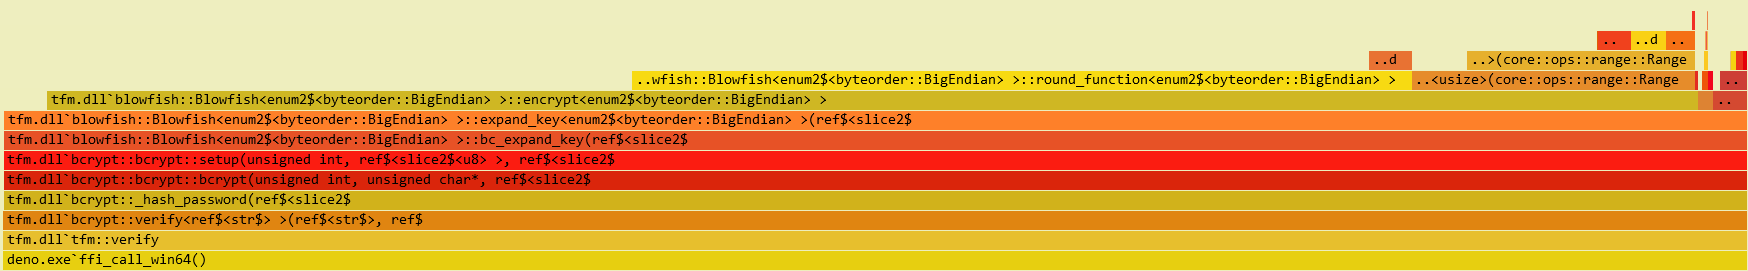
\includegraphics[width=\textwidth]{flamegraph}
    \caption{Flamegraph of the verify function.}
    \label{img:flamegraph}
\end{figure*}

\subsection{Where WASM fits}

WASM, as previously mentioned, is most suitable for the browser environment where it was designed to operate. Currently, it is still in its nascent stage, and the WASM API within the browser remains under development. While the WASI libc library is functional, it has yet to reach full maturity.

This is discussed in a GitHub issue. \cite{WASMBAD}

\begin{itemize}
    \item There's no way to control, in a guaranteed manner, when a new memory commit versus address space reserve takes place.
    \item There's no method to uncommit utilized memory pages.
    \item It's impossible to reduce the size of allocated Wasm Memory.
    \item Absence of virtual memory support, compelling applications to either always anticipate the ability to expand or to implement memory defragmentation solutions.
    \item If Memory is shared, the application must determine the maximum memory size in advance, or preemptively reserve as much as possible.
\end{itemize}

The author encapsulates the issue by stating, \textit{"you can only acquire more memory, without assurance if the memory acquired is reserved or committed"}.

In WASM, there's no method to allocate memory at compile time, which would have been advantageous for this project. This inability of WASM poses a significant constraint for this project and consequently, leads to suboptimal performance.

\subsection{The data}

Let's examine the actual data to determine if this idea holds true. These tests were conducted using strings from a collection of 36 characters, repeated from 1,000 to 2,000 times. Each set was repeated 15 times, and the average was calculated to eliminate potential errors.

The data was collected sequentially, ensuring that no async functions were used. The Deno and Rust functions were executed consecutively to minimize any noise introduced by the operating system.

\subsubsection{Hardware used}

These tests were run on a wide range of hardware, all of the \verb|x86_64| architecture.

\begin{itemize}
    \item GitHub Actions builders with a 2-core CPU \verb|x86_64| \cite{Github}
    \item i9-12900H
    \item i5-1135G7
\end{itemize}

The data presented in this document is sourced from the \textbf{i9-12900H} CPU. However, additional data can be found in the GitHub repository, extracted from every commit added to the repo.

Across all test runs, the results are consistent, albeit with expected speed differences given the diverse hardware selection.

The \textbf{i9-12900H} boasts a 16-core CPU with 24 threads. It operates with a base clock of 2.2 GHz and can boost up to 4.9 GHz. It possesses 24 MB of L3 cache and 16 MB of L2 cache. Being a robust CPU, it delivers impressive single-core performance. Consequently, this plays to Deno's advantage. Decreasing the speed of the processor would lead to increased time values for Deno.

\subsubsection{Hashing}

The initial part of the library to consider is hashing. Bcrypt is the algorithm employed for this purpose. Designed specifically for password hashing, bcrypt is deliberately slow to thwart brute-force attacks \cite{Bcrypt}. The algorithm's "cost" can be adjusted, which refers to the number of iterations it will undergo. A higher cost means a more secure hash but at the cost of time. Additionally, bcrypt incorporates a salt to deter rainbow table attacks.

\begin{figure}[H]
    \centering
    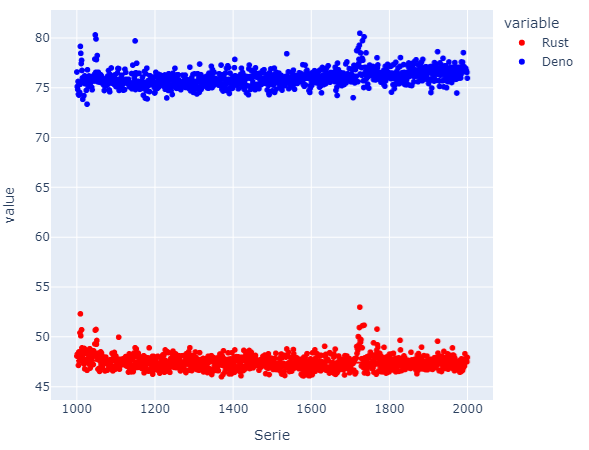
\includegraphics[width=0.52\textwidth]{hashing_lines}
\end{figure}

This image illustrates the creation of 1,000 hashes along with their respective costs in milliseconds, using a bcrypt cost of 14. On average, Rust is faster by \textbf{57\%}. When the hardware choice is limited to \textbf{i5-1135G7}, Deno's performance is \textbf{34\%} slower compared to Rust. Further limiting the hardware to a single-core instance of a VM running on DigitalOcean makes the disparity even starker, with Deno slowing down by \textbf{58\%} relative to Rust. These outcomes align with the findings from other tests conducted.

In the hash graph, a slight OS-induced noise is observable. This noise, evident at the beginning of the series and between 1600 and 1800, is not attributed to either Deno or Rust. Such anomalies can be excluded from the subsequent analysis.
The trends are not explicitly delineated, yet the subsequent graphs highlight two distinct aspects.

\begin{figure}[H]
    \centering
    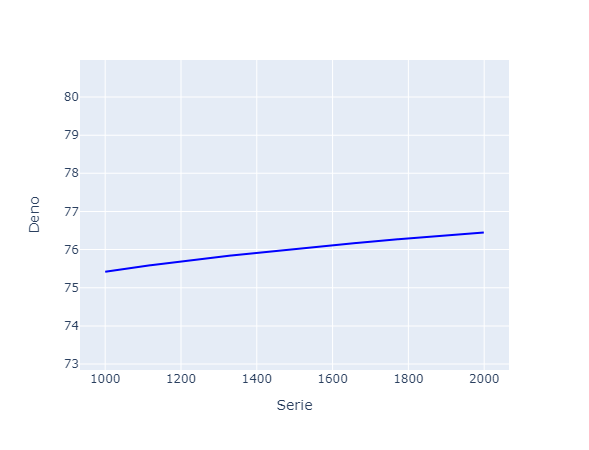
\includegraphics[width=0.52\textwidth]{trend_hash_deno}
\end{figure}

\begin{figure}[H]
    \centering
    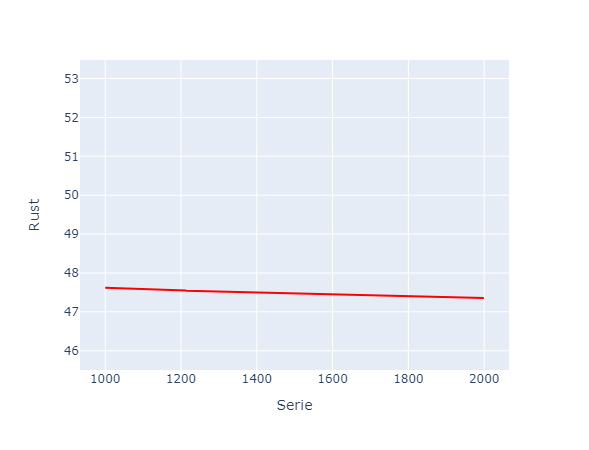
\includegraphics[width=0.52\textwidth]{images/trend_hash_rust.png}
\end{figure}

Several insights can be gleaned from the data:
\begin{itemize}
    \item The hashing cost in Deno escalates more swiftly than in Rust.
    \item Rust tends to be more stable, with a lesser increase in cost over time.
\end{itemize}

The growth rate in Deno is \textbf{0.001}, whereas in Rust, it's negligible for the data range chosen. Extending the character count to \textbf{1,800,000} leads to a growth rate of \textbf{0.0001} in Rust.

\subsubsection{Secret boxes}

Secret boxes are a concept introduced by the NaCl library. A secret box can be envisioned as a box with a single lock, acting as a metaphor for synchronous cryptography. For this project, the chosen algorithm is a variant named \textit{tweetnacl}. It mirrors the exact functionality of NaCl but can be encapsulated within 100 tweets.

The library's primary objectives are speed and a minimal disk footprint for both developers and end-users.

\begin{figure}[H]
    \centering
    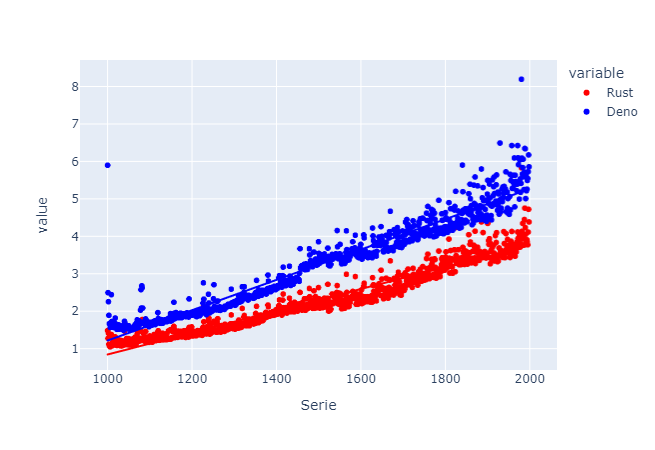
\includegraphics[width=0.52\textwidth]{images/secretbox_lines}
\end{figure}

In the depicted graph, certain Deno results diverge from the anticipated patterns. Given that these anomalies are absent in the Rust variant, they most likely originate from variations in V8's \textit{heat} function. Within V8, when a function is invoked, it accumulates \textit{heat}, implying that it's cached for subsequent calls. If a function is invoked repetitively, it's translated to machine code to optimize performance.

In this analysis, the relative instability of JavaScript compared to Rust is evident. Moreover, JavaScript appears to manifest a steeper increase in computational costs.

\begin{figure}[H]
    \centering
    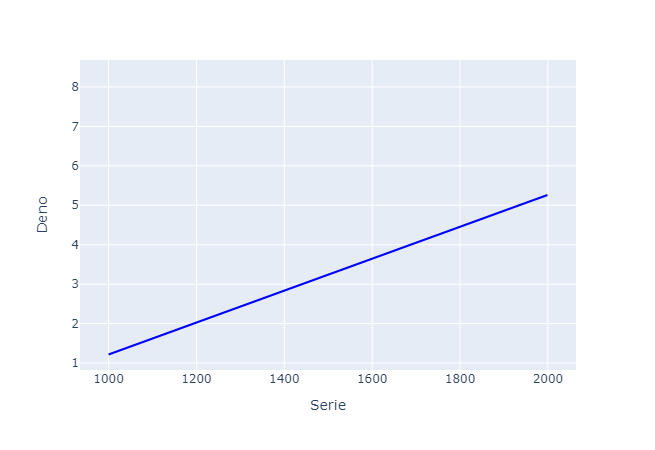
\includegraphics[width=0.52\textwidth]{trend_secretbox_deno}
\end{figure}

\begin{figure}[H]
    \centering
    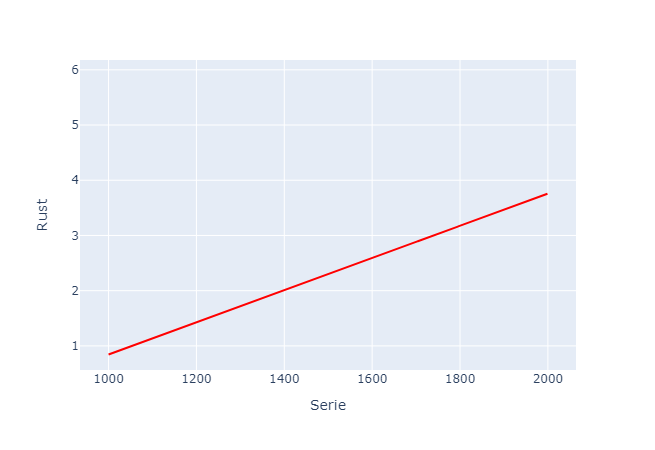
\includegraphics[width=0.52\textwidth]{images/trend_secretbox_rust}
\end{figure}

Several conclusions can be drawn from the data:
\begin{itemize}
    \item The cost of encryption escalates more swiftly in JavaScript than in Rust.
    \item Rust displays greater stability and experiences a milder growth in cost.
\end{itemize}

The growth rate in Deno stands at \textbf{0.004}, while in Rust it is \textbf{0.003}.

\subsubsection{Box}

A box can be envisioned as a container with two locks, serving as a metaphor for asymmetric encryption. Similar to the previous algorithm, this one is derived from \textit{tweetnacl}.

\begin{figure}[H]
    \centering
    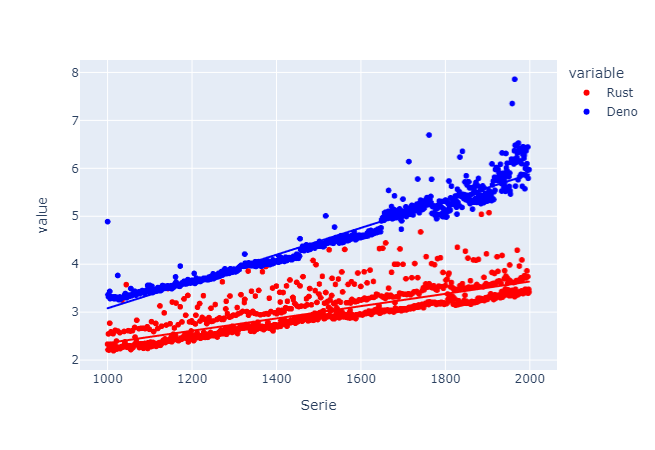
\includegraphics[width=0.52\textwidth]{images/box_lines}
\end{figure}

For this particular algorithm, Rust notably outperforms Deno, even if its results display a wider spread.

\begin{figure}[H]
    \centering
    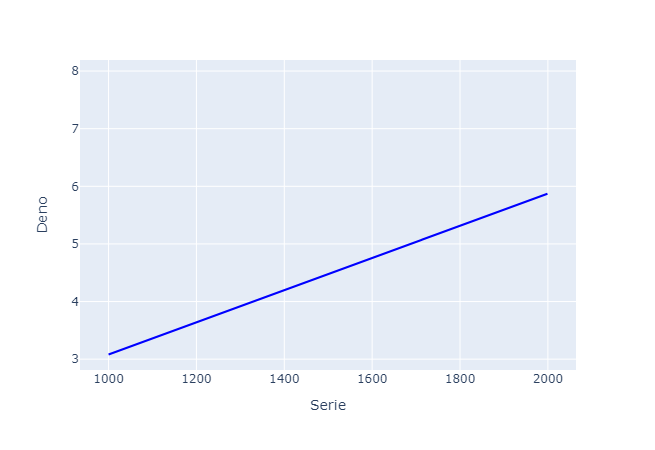
\includegraphics[width=0.52\textwidth]{trend_box_deno}
\end{figure}

\begin{figure}[H]
    \centering
    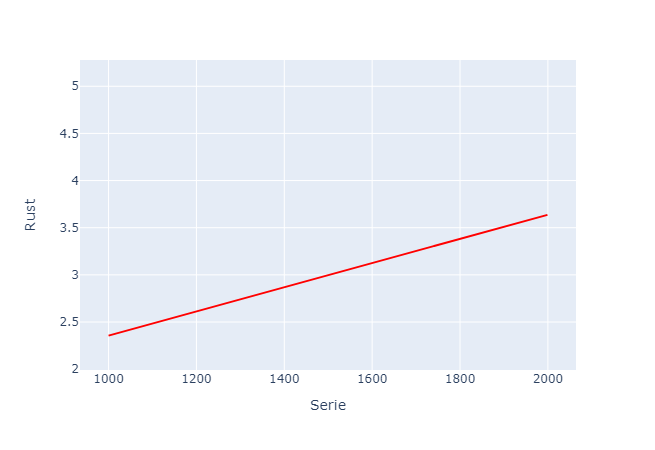
\includegraphics[width=0.52\textwidth]{images/trend_box_rust}
\end{figure}

From the presented data, the following observations can be made:
\begin{itemize}
    \item The cost of encryption escalates more swiftly in Deno compared to Rust.
    \item Rust demonstrates greater stability and a slower growth rate.
\end{itemize}

The growth rate for Deno is \textbf{0.003} and for Rust it is \textbf{0.001}.

\section{Conclusions}

The objective of this project has been achieved with significant success, both in theory and in practice. The primary motivation for this initiative was the necessity to improve the efficiency of JavaScript-based projects, a technology that continues to grow in ubiquity. A prominent application of this effort can be seen in the InterPlanetary File System (IPFS) \cite{IPFS}, which heavily depends on our optimized suite of algorithms for its operations. Specifically, this suite of libraries is fundamental to the functionality of OrbitDB, a crucial library used to establish decentralized databases.

\subsection{Technical Overview}

The libraries produced as part of this project are rooted in distributed technology paradigms. These paradigms hinge on a principle of data transmission involving multiple peers. In this setup, each peer dispatches fragments of data to a centralized entity. Given this architecture, the demand for swift data aggregation and dissemination becomes paramount. Such needs pose distinct challenges when relying on conventional methods of information transfer.

\subsection{Performance Limitations in IPFS}

Though IPFS is fundamentally based on JavaScript, it isn't spared from the typical performance challenges associated with the language. Even with the noteworthy optimization efforts by the IPFS development team, the system's potential is hindered by JavaScript's intrinsic limitations.

A significant advancement occurred when IPFS was implemented in the Go programming language, celebrated for its C Application Binary Interface (ABI) and potent WebAssembly (WASM) capabilities. However, the core functionalities continue to lean on JavaScript. While various IPFS protocol implementations exist, the official one remains the most widely adopted, leading to pronounced network latency.

\subsection{Performance Augmentation}

Integrating our library is expected to markedly enhance performance metrics in both desktop applications and web-based environments.

\subsection{Future-Proofing Developer Environments}

In this project, emphasis is placed on the utilization of Deno due to its sandboxed nature. The subsequent step in safeguarding against execution of malevolent code on developer machines would be to adopt containers. This ensures that the executed code remains benign. Employing Docker containers for this purpose provides a consistent and reproducible development environment, complete with essential dependencies. It also acts as a security buffer, with the working codebase ensconced within a contained setting, effectively mitigating potential hazards.

\subsection{Industry Leadership}

Microsoft stands as a pioneer in this technological realm, especially with their groundbreaking feature in Visual Studio Code called Remote Containers. This tool allows developers to run code within a containerized setting directly from a designated folder, eliminating the need for local dependency installations. Not only is this feature beneficial for enriching the developer experience, but it's also pivotal for strengthening security measures.

Microsoft furnishes a local variant of this utility, termed \verb|dev-containers|, which offers the same features but functions within a local environment.

\bibliographystyle{unsrt} % We choose the "plain" reference style
\bibliography{refs} % Entries are in the refs.bib file
\end{document}